\chapter{Introduction}
Proteins are biological macromolecules that perform a large variety of functions in living cells comprising biochemical (enzymes), structural, mechanical, and signaling functions. They consist of chains composed of 20 different natural amino-acids. To perform their functions, proteins interact with small molecules referred to as ligands, which are able to bind to a protein with high affinity and specificity \cite{du2016insights}. These protein/ligand interactions are crucial in biology, particularly in the context of drug design \cite{li2019predicting}. Since proteins interact with a broad range of drugs, it is of particular interest to study their flexibility and the mechanisms of binding of ligands to proteins and its impact on the structural dynamics to gain insights into:
\begin{itemize}
	\item Phenomena involved in the biological processes and related to diseases \cite{silva2010ligand} such as misfolding disease or aggregation
	\item Discovery, design, and development of new drugs \cite{payandeh2021ligand}.
\end{itemize}
 The atomic structural data provide key structural information of the ligand-bound and ligand-unbound (APO) proteins \cite{chakraborti2021all}. \textbf{Nevertheless, the static information is not sufficient for understanding protein–ligand binding mechanisms, especially when pockets are highly flexible and contain several binding sites}. Therefore, molecular modeling and simulations such as Molecular Dynamics (MD) or Normal Mode Analysis (NMA) are powerful tools that provides a description of the dynamics and structures of protein–ligand systems with a high spatial and temporal resolution.
 
 \section{3-D structures of proteins and the AlphaFold revolution}
 
 As explained above, proteins are essential biological macromolecules and the resolution of their three-dimensional (3-D) structure is crucial to understand their biological functions. For many years, considerable efforts have been made to resolve experimentally atomic structures of proteins using X-ray Diffrection (XRD), Nuclear Magnetic Resonance (NMR), or Cryo-Electron Microscopy (Cryo-EM). To date, around 200,000 3-D structuyres of proteins have been resolved experimentally and deposited in a database named Protein Data Bank (PDB, \url{https://www.rcsb.org}). However, it represents only a small fraction of resolved structures compared with the hundreds of billions of sequences of proteins referenced in the Universal Protein Resource (UniProt, \url{https://www.uniprot.org}) sequence database. This limitation is essentially due to the experimental constraints and exhaustive protocols that need to be performed to resolve such flexible structures, as presented in Table~\ref{TAB1}.
 
 \begin{table}[h!]
 	\begin{tabular}{cp{4cm}p{5cm}p{4.5cm}}
 		\hline
 		 & Advantages & Disadvantages & Macromolecules\\
 		 \hline
 		 \multirow{4}{*}{XRD} & • Well developed & • Crystallization process & • Soluble proteins \\
 		  & • High resolution & • Diffraction process
 		   & • Proteins complexes \\
 		  & • Broad MW range & • Solid structure preferred & • Membranes, Ribosomes \\
 		  & • Model building &• Static crystalline structure & • DNA/RNA \\
 		  \hline
 		 \multirow{3}{*}{NMR} & • High resolution & • High sample purity & • MWs below 40–50 kDa \\
 		 & • Structure in solution & • Sample preparation & • Water soluble samples\\
 		 & • Dynamic study	& • Computational simulation & \\
 		 \hline
 		 \multirow{3}{*}{Cryo-EM} & • Sample preparation & • Relatively low resolution
 		  & • MWs > 150 kDa\\
 		 & • Native state & • Highly dependent on EM & • Large proteins\\
 		 & • Small sample size	& • EM equipment & • Complex compounds \\
 		 \hline
 	\end{tabular}
 	\caption{The comparison of X-ray crystallography, NMR and Cryo-EM. MW acrocym refers to molecular weight.}
 	\label{TAB1}
 \end{table}
 
 Therefore, being able to predict the 3-D structure of a protein from its sequence of amino acid, \textit{i.e.} the folding phenomenon, is very challenging. This has presented a formidable computational challenge for many decades. Two years ago, a significant advance was announced by DeepMind, a London-based Artificial Intelligence (AI) company now part of Google’s parent firm. They developed a AI program named AlphaFold\cite{AlphaFold} that was able to predict of protein 3-D structures with an accuracy competitive with experiments. Therefore, AlphaFold has the potential to revolutionize the way one consider the design of biosystems, allowing to predict 3-D structures of proteins that have not yet been experimentally characterized.
 
 Basically, The AlphaFold network directly predicts the 3D coordinates of all heavy atoms for a given protein using the primary amino acid sequence and aligned sequences of homologues as input (Fig.~\ref{FIG1}). AlphaFold extracts data from two major databases, \textit{i.e.} genetic and structure (PDB) datasets and uses novel neural network architectures and training procedures based on the evolutionary, physical and geometric constraints of protein structures. The architecture jointly embed multiple sequence alignment (MSA, see section X) and pairwise features (2-D arrays). Then, the data processed through a network comprised of two main stages, called Evoformer and Structure module. More details about AI architectures of these twi networks can be found here~\cite{AlphaFold}.
 
 \begin{figure}[h!]
 	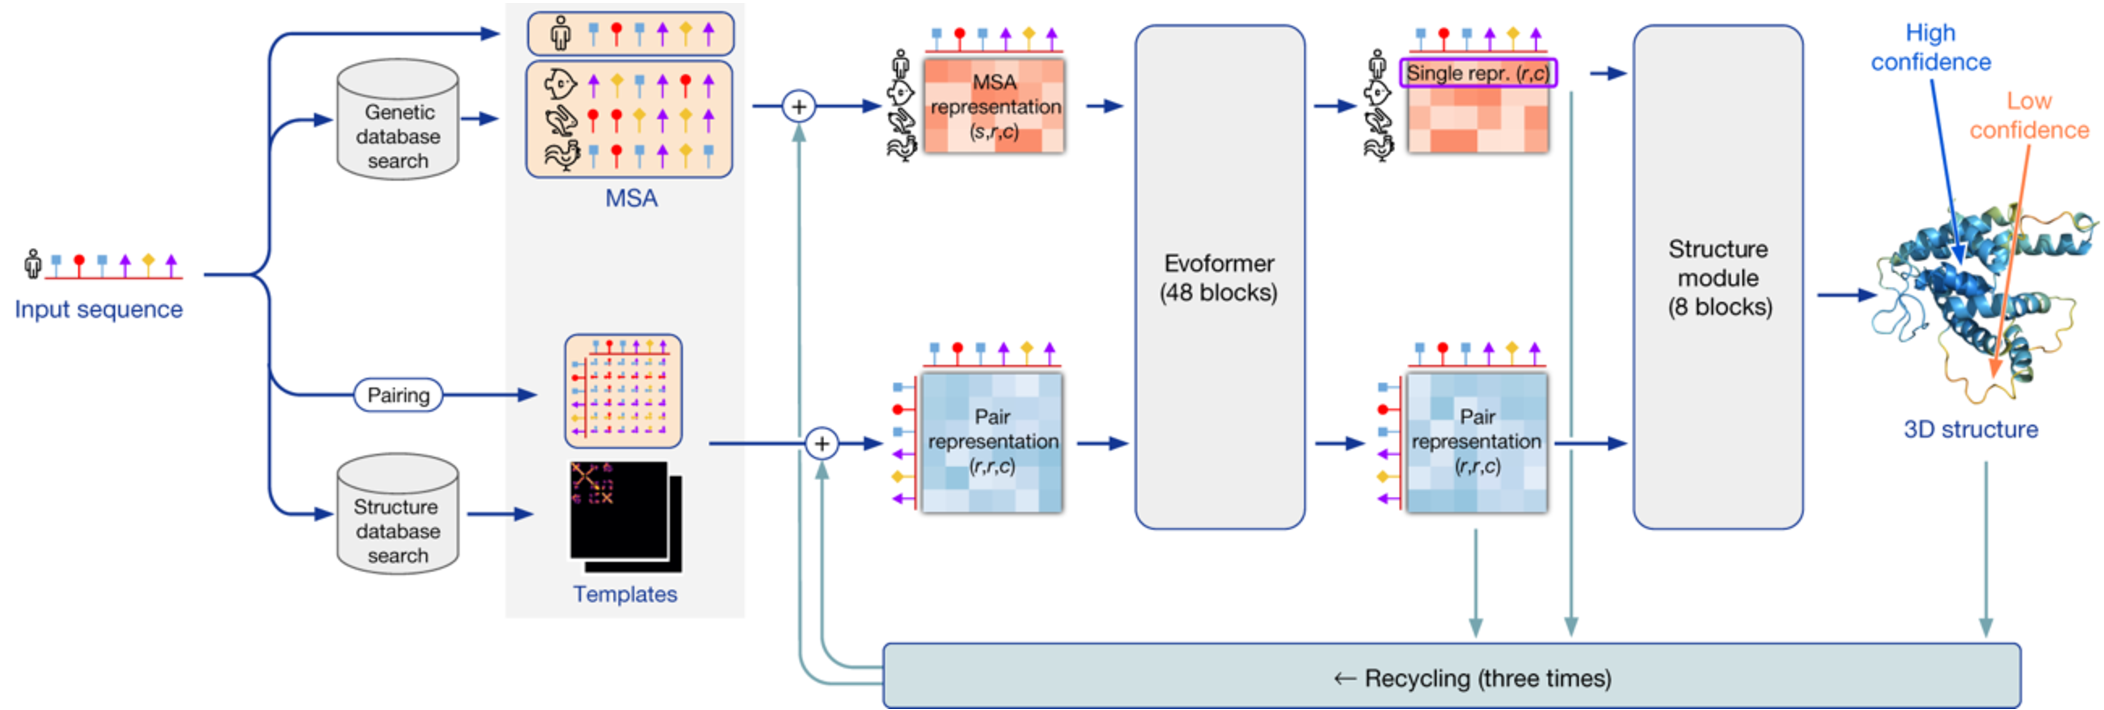
\includegraphics[width=16cm]{../figures/figure_AF_scheme.pdf}
 	\caption{Model architecture of AlphaFold program. Arrows show the information flow among the various components. The figure was extracted from reference~\cite{AlphaFold}.}
 	\label{FIG1}
 \end{figure}
  
  \textbf{This major breakthrough in the structural biology community will aid fundamental research for a better understanding of biological phenomena and for the development of applications in medical or environmental research.}
 
\section{Glutathione Transferase}
Glutathione transferases (GSTs) belong to a ubiquitous superfamily of enzymes that
metabolize a broad range of reactive toxic compounds by catalyzing the conjugation of reduced tripeptide glutathione ($\gamma$-Glu-Cys-Gly; named GSH) to the electrophilic center of a second substrate \cite{mannervik1985isoenzymes, armstrong1997structure, hayes2005glutathione}, the reactivity of GSH being due to the thiol group SH of the cysteine residue. The conjugation reaction occurs spontaneously but GST accelerates it dramatically. This process of detoxification protects cells against damages caused by both exogenous and endogenous molecules. GSTs were first discovered in liver cells \cite{combes1961liver}, and since then, they have been found to exhibit ligand-binding properties for a large variety of compounds, which are not always their enzymatic substrates \cite{axarli2004characterization}. Therefore, GSTs participate in diverse biological processes, making them multifunctional proteins. Moreover, GSTs are classified into three families according to their location in the cell: cytosolic, mitochondrial, and microsomal, which is not evolutively related to the two other classes \cite{oakley2011glutathione}. First-discovered and most-abundant cytosolic GSTs are divided into 13 classes based on homology of their sequences.Members of the same cytosolic class have at least $40\%$ of sequence identity, while members of different classes must have at most $25\%$ of sequence identity. 

 \begin{figure}[b!]
	\includegraphics[width=12.5cm]{../figures/figure_GST.pdf}
	\caption{A. Cartoon representation of GSTA1 monomer structures. Left panel: subdomains (I) and (II) are indicated in magenta and red, respectively. Right panel: the color code is the following: N-term (blue) to C-term (red). Secondary structures labels are also indicated. B. Ligand binding G (top panel) and H (bottom panel) sites of GSTA1. Ligands are shown in green spheres and residues belonging to the binding sites are shown in yellow and purple sticks, respectively. The color code is the following: GSTA1 monomer A in red, GSTA1 monomer B in blue. C. Catalytic cycle of GSH conjugation to electrophilic substrate. 3 forms of GSTA1 during the conjugation reaction cycle are highlighted: APO (no compound bound), GSH (Glutathione bound) and GS-R (Gluthatione-S-conjugated substrate). The R form (substrate bound) is not considered in the present work. The color code is the same as in panel B.}
	\label{FIG2}
\end{figure}

With some exceptions, GSTs are catalytically active as dimers. GST monomers are, in general, made of 200 to 250 residues with a molecular weight generally comprised between 25 and 30 kDa~\cite{frova_glutathione_2006,board_glutathione_2013} and are organized into two subdomains (Fig.~\ref{FIG2}A). The typically 80-residue-long N-terminal subdomain (I) has the typical fold of thioredoxin. It contains a first active site where GSH is hosted in catalytic conformation, named G site (Fig.~\ref{FIG2}B). The thioredoxin fold is composed of a characteristic sequence of $\alpha$-helices and $\beta$-strands encountered in the thioredoxin protein family, i.e. $\beta_1-\alpha_1-\beta_2-\alpha_2-\beta_3-\beta_4-\alpha_3$, which is characteristic of enzymes dealing with gluthatione such as glutaredoxin or glutathione peroxydase~\cite{atkinson_atlas_2009}. In addition, it has been shown that the region $\beta_3-\beta_4-\alpha_3$ is well conserved among GSTs and enables GSH recognition by the enzyme~\cite{armstrong_structure_1997}. Residues forming the G site (Fig.~\ref{FIG2}B) are generally conserved among GSTs~\cite{board_glutathione_2013}. A noticeable exception is the residue of $\alpha_1$-helix which interacts with the sulfur atom of GSH and which can be a Cysteine, a Serine, or a Tyrosin. Depending on the nature of this residue, GSTs develop slightly different catalytic functions and target a different range of substrates~\cite{deponte_glutathione_2013}. The second subdomain (II) is all-helical and contains the H site which binds the substrate. The number of helices varies between 4 and 7 among GSTs. Subdomain (II) is hydrophobic, and therefore attractive for hydrophobic molecules. Together with the G site, the combined architecture of GST monomers is adapted to bind GSH to hydrophobic substrates~\cite{mannervik_glutathione_1988}. Contrary to the G site (Fig.~\ref{FIG2}B), the residues of the H site strongly vary from one GST to the others, resulting in H sites of different natures and the ability to recognize different substrates~\cite{cummins_multiple_2011}. 

Finally, Fig.~\ref{FIG2}C presents the conjugation reaction cycle of GST enzymes. During this reaction, GSTs exist in three different forms: i) the APO form, when there is no compound bound to GST, ii) the GSH form, when the glutathione is bound to the G-site and iii) the GS-R form, when the glutathione-S-conjugated substrate is bound to the G and H site. Another existing form of GST enzymes is not shown here, \textit{i.e.} the R form (substrate bound). Indeed, the binding of the gluthatione ligand and of the substrate is not sequential. The substrate can bind first to GST and then the GSH or the opposite way, as presented in Fig.~\ref{FIG2}C. 

\section{Goal of the present work}

In the present work, we focus our interest to the GSTs identified in \textit{Drosophila melanogaster}. It corresponds to 42 structures in total with the $\delta$ and $\varepsilon$ that are the largest classes, with 25 members \cite{F-Neiers-GSTs}. Interactions between insects and plant’s chemicals lead to a major driving force in herbivorous insect evolution, hence this encourages the study of insect GSTs to understand how spontaneous mutations modify the stability, selectivity and the catalytic efficiencies of this enzyme family.
